\section{PROPOSED METHOD}
Our proposed model consists of two steps:
a) a CNN based model providing a coarse segmentation of synaptic cleft;
b) a contour growing algorithm that use the coarse segmentation to localize whole contours of synaptic cleft region.
The pipeline of our framework is illustrated in Figure~\ref{fig:cg}.

\begin{figure*}[t]
    \begin{center}
        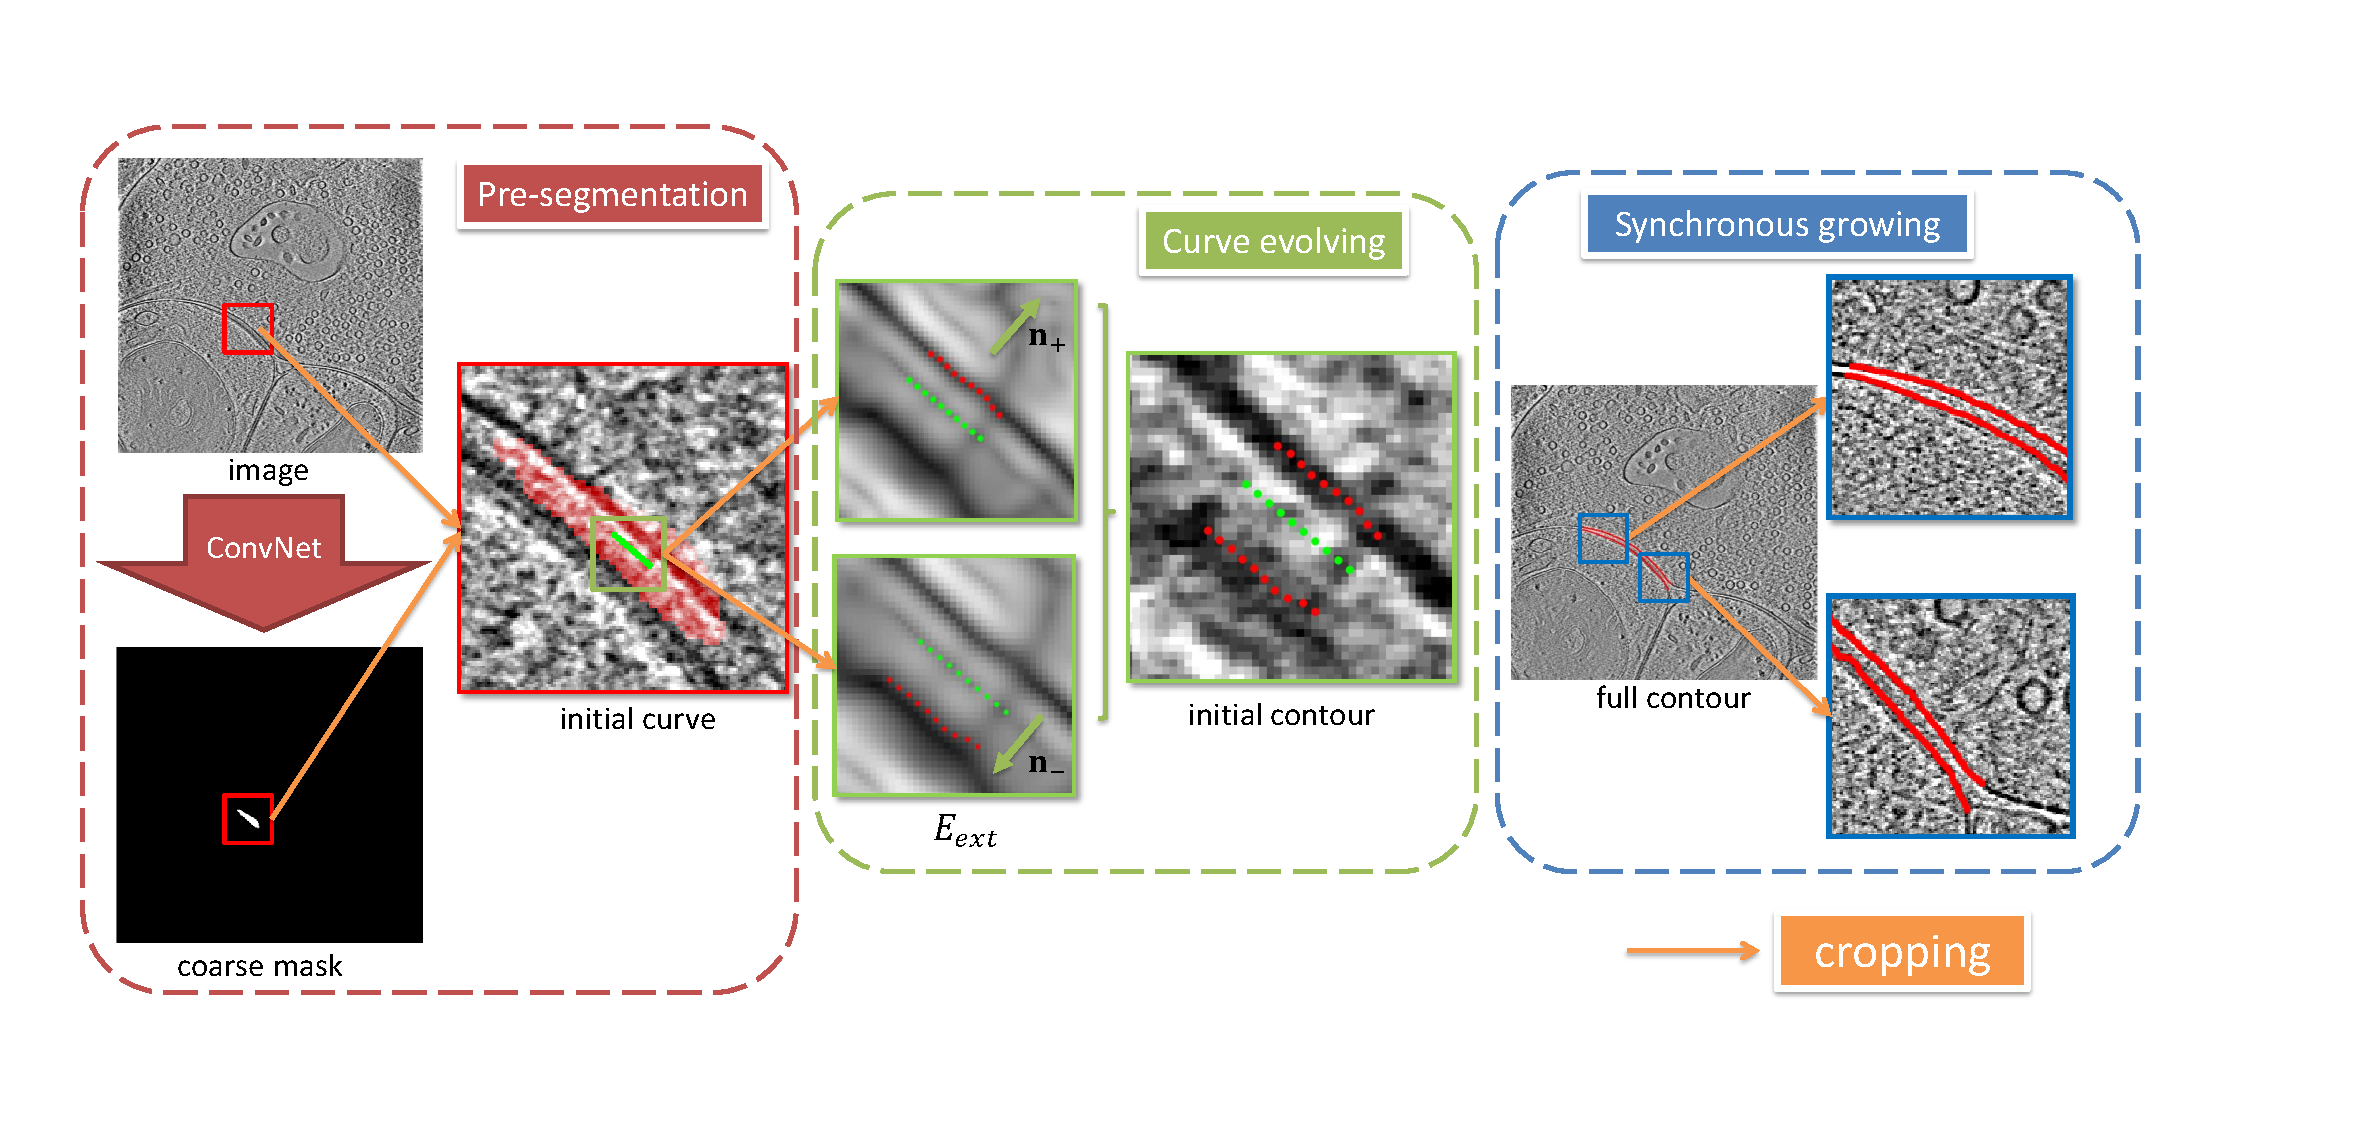
\includegraphics[width=7in]{figs/FigCG.pdf}
   \end{center}
\caption{A brief view of our model in localizing the synaptic cleft region. First a CNN based model results in a coarse segmentation mask, which provides an initial curve (green line) in cleft region.
        Then, the initial curve is respectively evolved along opposite direction ($\mathbf{n}_+$ and $\mathbf{n}_-$) to obtain two piece of initial contours (red dotted line).
        Finally, we will synchronously grow the contours to localize the whole synaptic cleft region (encircled by red solid curves).}
\label{fig:cg}
\end{figure*}

\subsection{Pre-segmentation}
To accurately localize the location of our target regions, deep convolutional networks are first implemented to give a coarse segmentation for synaptic cleft.
The architecture of the networks are based on famous DeepLab \cite{Chen2016a}, which uses the dilated convolution for lager reception field.
Differently, we change the classifier of DeepLab to be a binary classifier and use a weighted loss for mitigating unbalanced label problem in our task.
For the problem of limited data caused by expensive acquisition, the transfer learning strategy is used by fine-tuning the weights of lower layers on the off-the-shelf model from DeepLab, which has been well trained on natural images.

\subsection{Contour growing algorithm}
\subsubsection{curve evolving}
\label{sec:curve_evolving}
Based on the binary mask from pre-segmentation, we first generate an initial curve from the mask, which will be subsequent evolved to attach to the target contour.
In order to make sure that the initial curve is inside the cleft region, it will be generated as short as possible, such as the green dotted line in Figure~\ref{fig:cg}.
Then the initial curve will be evolved twice to respectively attach to presynaptic and postsynaptical membranes, which are exactly the contours of synaptic cleft.

Similar to the traditional snake model \cite{Kass1988}, the initial curve is expressed by $\mathbf{v}(s)=[x(s),y(s)]$, where $s\in[0,1]$, and our goal is to minimize the following energy function:
\begin{eqnarray}\label{Eq:Etotal}
E_{total} =& \int_{0}^{1}[E_{int}\{\mathbf{v}(s)\}+E_{ext}\{\mathbf{v}(s)\}]ds\nonumber \\
E_{int} =& \int_{0}^{1}[\alpha\{\mathbf{v}^{'}(s)\}+\beta\{\mathbf{v}^{''}(s)\}]ds \\
E_{ext} =& \int_{0}^{1}[I\{\mathbf{v}(s)\} + \kappa G\{\mathbf{v}(s)\}]ds\nonumber
\end{eqnarray}
where $\mathbf{v}^{'}(s)$ and $\mathbf{v}^{''}(s)$ are respectively the first and second derivative of $\mathbf{v}(s)$.
$I$ is the Gaussian smoothed image.
$G$ is the gradient magnitude map.
According to \cite{Kass1988}, minimizing Eq.~\ref{Eq:Etotal} can be obtained by iteratively updating the following equations:
\begin{eqnarray}\label{Eq:GVF}
\mathbf{v}_{t+1}(s) = (A+\gamma I)^{-1}(\gamma \mathbf{v}_t(s)+\mathbf{f}\{x_t(s)\})
\end{eqnarray}
where $A$ is a matrix representing the internal tension, $\gamma$ controls the evolving rate and $\mathbf{f}=[f_{x},f_{y}]$ are the gradient maps calculated from $E_{ext}$ using Gradient Vector Flow (GVF) algorithm \cite{Xu1998}.

However Eq~\ref{Eq:GVF} is very sensitive to noisy regions, which easily trap some control points.
Furthermore the capture range of tension $\mathbf{f}$ is usually limited \cite{Cohen1991}, making its performance depend heavily on initial curve.
Our experiments illustrate the deficiencies of GVF in detail and show some representative cases in Figure~\ref{fig:gvf}.
Therefore, we propose a new updating strategy by:
\begin{eqnarray}\label{Eq:update}
\mathbf{v}_{t+1}(s) = (A+\gamma I)^{-1}(\gamma \mathbf{v}_t(s)+E_{ext}\{\mathbf{v}(s)\}\mathbf{n}\{\mathbf{v}_t(s)\})
\end{eqnarray}
$\mathbf{n}\{\mathbf{v}(s)\}$ are the normal vectors of $\mathbf{v}(s)$ with consistent orientations.

In Eq.~\ref{Eq:update}, the direction of external tension are fixed as the normal direction of $\mathbf{v}_(s)$, whose magnitude are controlled by $E_{ext}\{\mathbf{v}(s)\}$ instead of a constant value in Ballons model \cite{Cohen1991}.
The advantages of Eq.~\ref{Eq:update} are follows:
a) the capture range of external tension are much larger, due to fixed tension $\mathbf{n}\{\mathbf{v}(s)\}$;
b) it is easier to reach the global optimum than GVF, because $E_{ext}$ will soon vanish in contour region;
c) In the noise region, once the internal tension pulls a trapped $\mathbf{v}(s)$ out, our external tension will soon push it away.
The above situations are shown in Figure~\ref{fig:gvf}.

By setting opposite normal vectors ($\mathbf{n}_{+}$ and $\mathbf{n}_{-}$ in Figure~\ref{fig:cg}), $\mathbf{v}(s)$ will be evolved along opposite direction and well attach to both presynaptic and postsynaptical membranes.
The final evolved curves are respectively denoted as $\mathbf{c}_1(s)$ and $\mathbf{c}_2(s)$

\begin{figure}[t]
\begin{minipage}[b]{1.0\linewidth}
  \centering
 \centerline{\epsfig{figure=Figs/FigG.pdf,width=8.5cm}}
\end{minipage}
\caption{An example of contour growing formulated by Eq.~\ref{Eq:sg}.
        The yellow solid array indicate the growing direction of last stage.
        The dotted arrays give several candidates of next growing direction, while the one with the deepest color are preferred.
        After finding the optimal length, the longest array are chosen as a new piece of growing contour.}
\label{fig:g}
\end{figure}

\begin{figure}[t]
\begin{minipage}[b]{1.0\linewidth}
  \centering
 \centerline{\epsfig{figure=Figs/FigSG.pdf,width=8.5cm}}
\end{minipage}
\caption{Diagram of different situations illustrated in Eq.~\ref{Eq:gf}.
        The green line is the new growing contour, while the red line is the previous contour}
\label{fig:sg}
\end{figure}
\subsubsection{synchronous growing}
With two pieces of contour $\mathbf{c}_1(s)$ and $\mathbf{c}_2(s)$, we then grow them to localize the whole presynaptic and postsynaptic membranes.
The challenge of this part is that they should be grown correctly and synchronously to compute the exact distance between two membranes for termination judging.

First, we formulate the process of growing $\mathbf{c}_1(s)$ as finding a piece of line $\mathbf{l}(s)$ by:
\begin{eqnarray}\label{Eq:sg}
&\arg\min_{\mathbf{l}(s)} E_{int}\{\mathbf{l}(s)+c_1(1))\}+\rho(\overrightarrow{c_1}(1)*\overrightarrow{l}(0))\\
&st. \tau_1\leq (\overrightarrow{c_1}(0)*\overrightarrow{l}(0))\leq \tau_2\nonumber
\end{eqnarray}
where $c_1(1)$ is the end point of curve $\mathbf{c}_1$ and $\overrightarrow{c_1}(0)$ is the tangent vector of point $c_1(1)$.
Especially, $\mathbf{l}(s)$ is straight and can be expressed by a direction vector $\overrightarrow{l}(0))$ and a length $l$.
And $*$ defines the inner product of two vectors.
The firs term of Eq.~\ref{Eq:sg} hope $\mathbf{l}(s)$ to be inside the membrane, while the second term hope the growing direction to follow the previous growing direction.
$\rho$ is a tradeoff parameter, and $\tau_1,\tau_2$ add a hard restraint on the growing direction to be not changed too much.

Optimal solution of Eq.~\ref{Eq:sg} can be obtained by using EM algorithm.
Explicitly, we first fixed $l$ to find an optimal $\overrightarrow{l}(0))$, and then fix $\overrightarrow{l}(0))$ to find a better $l$.
Experiments show that two times of iteration is enough for most cases to give a satisfying piece of new growing membrane as shown in Figure~\ref{fig:g}.

Next to synchronously grow $\mathbf{c}_1(s)$ and $\mathbf{c}_2(s)$, we split the growing process into several periods and decide which curve grows in each period.
Especially, we set two variables $g_1^{t+1}$ and $g_2^{t+1}$ to determine the growing state of $\mathbf{c}_1^{t}(s)$ and $\mathbf{c}_2^{t}(s)$ at stage $t+1$ by:
\begin{eqnarray}\label{Eq:gf}
g_1^{t+1},g_2^{t+1} = \left\{\begin{array}{cc}
0,1&if \overrightarrow{c}^t_1(1)*(c_2^t(1)-c_1^t(1))\geq 0 \\
1,0&if \overrightarrow{c}^t_1(1)*(c_2^t(1)-c_1^t(0))\leq 0\\
1,1& else\\
\end{array}\right.
\end{eqnarray}
where $c_1^t(0)$, $c_1^t(1)$ and $c_2^t(1)$ are three endpoints of two growing membranes as shown in Figure~\ref{fig:sg}, of which the positions determine $g_1^{t+1}$ and $g_2^{t+1}$ ($1$ for growing and $0$ for waiting).
Different situations of Eq.~\ref{Eq:gf} are shown in Figure~\ref{fig:sg}.
The distance between two membranes can be calculated by:
\begin{eqnarray}\label{Eq:d}
d^{t+1} = \frac{||c_1^{t+1}(1)-c_2^{t+1}(1)||+ ||c_1^{t+1}(0)-c_2^{t+1}(0)||}{2}
\end{eqnarray}
Once $d^{t+1}$ is beyond the range of reasonable cleft width, the growing will be terminated.
